\documentclass{ximera}

%\usepackage{todonotes}

\newcommand{\todo}{}

\usepackage{esint} % for \oiint
\ifxake%%https://math.meta.stackexchange.com/questions/9973/how-do-you-render-a-closed-surface-double-integral
\renewcommand{\oiint}{{\large\bigcirc}\kern-1.56em\iint}
\fi


\graphicspath{
  {./}
  {ximeraTutorial/}
  {basicPhilosophy/}
  {functionsOfSeveralVariables/}
  {normalVectors/}
  {lagrangeMultipliers/}
  {vectorFields/}
  {greensTheorem/}
  {shapeOfThingsToCome/}
  {dotProducts/}
  {partialDerivativesAndTheGradientVector/}
  {../productAndQuotientRules/exercises/}
  {../normalVectors/exercisesParametricPlots/}
  {../continuityOfFunctionsOfSeveralVariables/exercises/}
  {../partialDerivativesAndTheGradientVector/exercises/}
  {../directionalDerivativeAndChainRule/exercises/}
  {../commonCoordinates/exercisesCylindricalCoordinates/}
  {../commonCoordinates/exercisesSphericalCoordinates/}
  {../greensTheorem/exercisesCurlAndLineIntegrals/}
  {../greensTheorem/exercisesDivergenceAndLineIntegrals/}
  {../shapeOfThingsToCome/exercisesDivergenceTheorem/}
  {../greensTheorem/}
  {../shapeOfThingsToCome/}
  {../separableDifferentialEquations/exercises/}
  {vectorFields/}
}

\newcommand{\mooculus}{\textsf{\textbf{MOOC}\textnormal{\textsf{ULUS}}}}

\usepackage{tkz-euclide}
\usepackage{tikz}
\usepackage{tikz-cd}
\usetikzlibrary{arrows}
\tikzset{>=stealth,commutative diagrams/.cd,
  arrow style=tikz,diagrams={>=stealth}} %% cool arrow head
\tikzset{shorten <>/.style={ shorten >=#1, shorten <=#1 } } %% allows shorter vectors

\usetikzlibrary{backgrounds} %% for boxes around graphs
\usetikzlibrary{shapes,positioning}  %% Clouds and stars
\usetikzlibrary{matrix} %% for matrix
\usepgfplotslibrary{polar} %% for polar plots
\usepgfplotslibrary{fillbetween} %% to shade area between curves in TikZ
%\usetkzobj{all}
\usepackage[makeroom]{cancel} %% for strike outs
%\usepackage{mathtools} %% for pretty underbrace % Breaks Ximera
%\usepackage{multicol}
\usepackage{pgffor} %% required for integral for loops



%% http://tex.stackexchange.com/questions/66490/drawing-a-tikz-arc-specifying-the-center
%% Draws beach ball
\tikzset{pics/carc/.style args={#1:#2:#3}{code={\draw[pic actions] (#1:#3) arc(#1:#2:#3);}}}



\usepackage{array}
\setlength{\extrarowheight}{+.1cm}
\newdimen\digitwidth
\settowidth\digitwidth{9}
\def\divrule#1#2{
\noalign{\moveright#1\digitwidth
\vbox{\hrule width#2\digitwidth}}}




% \newcommand{\RR}{\mathbb R}
% \newcommand{\R}{\mathbb R}
% \newcommand{\N}{\mathbb N}
% \newcommand{\Z}{\mathbb Z}

\newcommand{\sagemath}{\textsf{SageMath}}


%\renewcommand{\d}{\,d\!}
%\renewcommand{\d}{\mathop{}\!d}
%\newcommand{\dd}[2][]{\frac{\d #1}{\d #2}}
%\newcommand{\pp}[2][]{\frac{\partial #1}{\partial #2}}
% \renewcommand{\l}{\ell}
%\newcommand{\ddx}{\frac{d}{\d x}}

% \newcommand{\zeroOverZero}{\ensuremath{\boldsymbol{\tfrac{0}{0}}}}
%\newcommand{\inftyOverInfty}{\ensuremath{\boldsymbol{\tfrac{\infty}{\infty}}}}
%\newcommand{\zeroOverInfty}{\ensuremath{\boldsymbol{\tfrac{0}{\infty}}}}
%\newcommand{\zeroTimesInfty}{\ensuremath{\small\boldsymbol{0\cdot \infty}}}
%\newcommand{\inftyMinusInfty}{\ensuremath{\small\boldsymbol{\infty - \infty}}}
%\newcommand{\oneToInfty}{\ensuremath{\boldsymbol{1^\infty}}}
%\newcommand{\zeroToZero}{\ensuremath{\boldsymbol{0^0}}}
%\newcommand{\inftyToZero}{\ensuremath{\boldsymbol{\infty^0}}}



% \newcommand{\numOverZero}{\ensuremath{\boldsymbol{\tfrac{\#}{0}}}}
% \newcommand{\dfn}{\textbf}
% \newcommand{\unit}{\,\mathrm}
% \newcommand{\unit}{\mathop{}\!\mathrm}
% \newcommand{\eval}[1]{\bigg[ #1 \bigg]}
% \newcommand{\seq}[1]{\left( #1 \right)}
% \renewcommand{\epsilon}{\varepsilon}
% \renewcommand{\phi}{\varphi}


% \renewcommand{\iff}{\Leftrightarrow}

% \DeclareMathOperator{\arccot}{arccot}
% \DeclareMathOperator{\arcsec}{arcsec}
% \DeclareMathOperator{\arccsc}{arccsc}
% \DeclareMathOperator{\si}{Si}
% \DeclareMathOperator{\scal}{scal}
% \DeclareMathOperator{\sign}{sign}


%% \newcommand{\tightoverset}[2]{% for arrow vec
%%   \mathop{#2}\limits^{\vbox to -.5ex{\kern-0.75ex\hbox{$#1$}\vss}}}
% \newcommand{\arrowvec}[1]{{\overset{\rightharpoonup}{#1}}}
% \renewcommand{\vec}[1]{\arrowvec{\mathbf{#1}}}
% \renewcommand{\vec}[1]{{\overset{\boldsymbol{\rightharpoonup}}{\mathbf{#1}}}}

% \newcommand{\point}[1]{\left(#1\right)} %this allows \vector{ to be changed to \vector{ with a quick find and replace
% \newcommand{\pt}[1]{\mathbf{#1}} %this allows \vec{ to be changed to \vec{ with a quick find and replace
% \newcommand{\Lim}[2]{\lim_{\point{#1} \to \point{#2}}} %Bart, I changed this to point since I want to use it.  It runs through both of the exercise and exerciseE files in limits section, which is why it was in each document to start with.

% \DeclareMathOperator{\proj}{\mathbf{proj}}
% \newcommand{\veci}{{\boldsymbol{\hat{\imath}}}}
% \newcommand{\vecj}{{\boldsymbol{\hat{\jmath}}}}
% \newcommand{\veck}{{\boldsymbol{\hat{k}}}}
% \newcommand{\vecl}{\vec{\boldsymbol{\l}}}
% \newcommand{\uvec}[1]{\mathbf{\hat{#1}}}
% \newcommand{\utan}{\mathbf{\hat{t}}}
% \newcommand{\unormal}{\mathbf{\hat{n}}}
% \newcommand{\ubinormal}{\mathbf{\hat{b}}}

% \newcommand{\dotp}{\bullet}
% \newcommand{\cross}{\boldsymbol\times}
% \newcommand{\grad}{\boldsymbol\nabla}
% \newcommand{\divergence}{\grad\dotp}
% \newcommand{\curl}{\grad\cross}
%\DeclareMathOperator{\divergence}{divergence}
%\DeclareMathOperator{\curl}[1]{\grad\cross #1}
% \newcommand{\lto}{\mathop{\longrightarrow\,}\limits}

% \renewcommand{\bar}{\overline}

\colorlet{textColor}{black}
\colorlet{background}{white}
\colorlet{penColor}{blue!50!black} % Color of a curve in a plot
\colorlet{penColor2}{red!50!black}% Color of a curve in a plot
\colorlet{penColor3}{red!50!blue} % Color of a curve in a plot
\colorlet{penColor4}{green!50!black} % Color of a curve in a plot
\colorlet{penColor5}{orange!80!black} % Color of a curve in a plot
\colorlet{penColor6}{yellow!70!black} % Color of a curve in a plot
\colorlet{fill1}{penColor!20} % Color of fill in a plot
\colorlet{fill2}{penColor2!20} % Color of fill in a plot
\colorlet{fillp}{fill1} % Color of positive area
\colorlet{filln}{penColor2!20} % Color of negative area
\colorlet{fill3}{penColor3!20} % Fill
\colorlet{fill4}{penColor4!20} % Fill
\colorlet{fill5}{penColor5!20} % Fill
\colorlet{gridColor}{gray!50} % Color of grid in a plot

\newcommand{\surfaceColor}{violet}
\newcommand{\surfaceColorTwo}{redyellow}
\newcommand{\sliceColor}{greenyellow}




\pgfmathdeclarefunction{gauss}{2}{% gives gaussian
  \pgfmathparse{1/(#2*sqrt(2*pi))*exp(-((x-#1)^2)/(2*#2^2))}%
}


%%%%%%%%%%%%%
%% Vectors
%%%%%%%%%%%%%

%% Simple horiz vectors
\renewcommand{\vector}[1]{\left\langle #1\right\rangle}


%% %% Complex Horiz Vectors with angle brackets
%% \makeatletter
%% \renewcommand{\vector}[2][ , ]{\left\langle%
%%   \def\nextitem{\def\nextitem{#1}}%
%%   \@for \el:=#2\do{\nextitem\el}\right\rangle%
%% }
%% \makeatother

%% %% Vertical Vectors
%% \def\vector#1{\begin{bmatrix}\vecListA#1,,\end{bmatrix}}
%% \def\vecListA#1,{\if,#1,\else #1\cr \expandafter \vecListA \fi}

%%%%%%%%%%%%%
%% End of vectors
%%%%%%%%%%%%%

%\newcommand{\fullwidth}{}
%\newcommand{\normalwidth}{}



%% makes a snazzy t-chart for evaluating functions
%\newenvironment{tchart}{\rowcolors{2}{}{background!90!textColor}\array}{\endarray}

%%This is to help with formatting on future title pages.
\newenvironment{sectionOutcomes}{}{}



%% Flowchart stuff
%\tikzstyle{startstop} = [rectangle, rounded corners, minimum width=3cm, minimum height=1cm,text centered, draw=black]
%\tikzstyle{question} = [rectangle, minimum width=3cm, minimum height=1cm, text centered, draw=black]
%\tikzstyle{decision} = [trapezium, trapezium left angle=70, trapezium right angle=110, minimum width=3cm, minimum height=1cm, text centered, draw=black]
%\tikzstyle{question} = [rectangle, rounded corners, minimum width=3cm, minimum height=1cm,text centered, draw=black]
%\tikzstyle{process} = [rectangle, minimum width=3cm, minimum height=1cm, text centered, draw=black]
%\tikzstyle{decision} = [trapezium, trapezium left angle=70, trapezium right angle=110, minimum width=3cm, minimum height=1cm, text centered, draw=black]


\title{Real Numbers}

\begin{document}

\begin{abstract}
dots and arrows
\end{abstract}
\maketitle



\textbf{$\mathbb{R}$} is not enough.  \\



Our investigation of the real numbers quickly expanded in many directions. We invented functions to help us see relationships within the real numbers.  However, this investigation also revealed shortcomings of the real numbers. The easiest example of which is that many quadratic polynomials cannot be factored using just the real numbers. Their roots are not real numbers. We need more numbers.


If we think of our history with numbers, we have encountered this idea of missing numbers many times.  We began with whole numbers, then expanded to include integers, then expanded to include rational numbers, and then expanded to include irrational numbers.  Each time, our picture was that the real line had unused spots and we were just filling in the picture.  However, the real line is now full. Whatever numbers we are missing are not real numbers.  There is no place for them on the real line.  Where are these new numbers coming from? More importantly, how are we going to represent these new numbers and keep track of which are new and which are the existing numbers?


\begin{idea} \textbf{\textcolor{purple!85!blue}{$\sqrt{-1}$}} \\


If we add $\sqrt{-1}$ to the real numbers, then we still want everything to work like it has been working.  We want our rules to continue working.


$\blacktriangleright$ We want addition to work : $\sqrt{-1} + \sqrt{-1} = 2\sqrt{-1}$ \\

$\blacktriangleright$ We want multiplication to work : $\sqrt{3} \cdot \sqrt{-1} = \sqrt{-3}$ \\


\end{idea}


If we throw $\sqrt{-1}$ in with $\mathbb{R}$ and let the rules tell us what else must be included, then it looks like $r\sqrt{-1}$ and $\sqrt{-r}$ will be included for every real number, $r$.  And, none of those numbers are currently in the real numbers. Our rules dictate that if we insert $\sqrt{-1}$, then we are forced to add in a whole new copy of $\mathbb{R}$.



It is feeling like we need two versions of real numbers. Maybe that is the answer. We just need two versions of the real numbers: the old real numbers and the new additonal real numbers.





\begin{center}
\textbf{\textcolor{purple!85!blue}{An immediate idea is to just use two copies of the real numbers.}}
\end{center}


In fact, we have been using two copies of the real numbers all along, just in a different context. Our graphs and curves on the Cartesian plane use two copies of the real numbers.  Each axis is a copy of the real numbers. We have been using the Cartesian plane to visually encode numbers as distances in an effort to illustrate the pairs in a function. Maybe we can repurpose the Cartesian plane to also have an algebraic structure - hopefully in a manner similar to how we use the real number. \\








We have a couple of tools we use to describe real numbers and our operations on them.


$\blacktriangleright$  We use written symbols to represent numbers and operations.  A string of valid symbols is called an expression and two expressions representing the same numbers are called equivalent. Accompanying these symbols are a list of manipulation rules and operations dictating how these symbols can be rearranged and replaced and yet still represent the same number.  We call this kind of communication Algebra.


$\blacktriangleright$  We also have diagrams that use space, direction, and size to visually represent numbers and operations. We call this diagram the real number line. Our line diagram has a line representing an ordering of the real numbers. Dots on the number line are one option for representing numbers, while arrows are often used to describe operations.


We would like to extend this system from one copy of \textbf{$\mathbb{R}$} to two copies of \textbf{$\mathbb{R}$}. \\



\begin{center}
\textbf{\textcolor{red!90!darkgray}{We would like to expand this number system from 1-dimension to 2-dimensions.}}
\end{center}







\section*{The Real Line:  $\mathbb{R}$}





Generally speaking we draw the real line horizontally with the negative numbers growing to the left and positive numbers growing to the right. Somewhere in the middle we draw a tick mark for $0$. We plot dots (points) on the real line at distances from $0$ that visually encode the value of the number.












  \begin{image}
  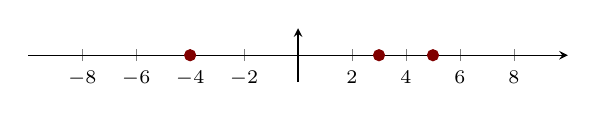
\begin{tikzpicture}
    \begin{axis}[
            xmin=-10,xmax=10,ymin=-1,ymax=1,
            %width=3in,
            clip=false,
            axis lines=center,
            %ticks=none,
            unit vector ratio*=1 1 1,
            ymajorticks=false,
            xtick={-8,-6,-4,-2,2,4,6,8},
            %xlabel=$x$, ylabel=$y$,
            ticklabel style={font=\scriptsize},
            %every axis y label/.style={at=(current axis.above origin),anchor=south},
            every axis x label/.style={at=(current axis.right of origin),anchor=west},
          ]     

            \addplot [color=penColor2,only marks,mark=*] coordinates{(-4,0)};
            \addplot [color=penColor2,only marks,mark=*] coordinates{(3,0)};
            \addplot [color=penColor2,only marks,mark=*] coordinates{(5,0)};




        \end{axis}
  \end{tikzpicture}
  \end{image}


Dots or points are a way of visually comparing numbers.  Bigger numbers are further from $0$, in either direction.  Greater numbers are to the right.  Lesser numbers are to the left.




Operations require something more than just dots. If we use arrows, then we can get both a signed numeric value from the arrow and the operations addition and subtraction from the arrow's placement.

Unlike dots, an arrow's position doesn't matter when representing a number. An arrow's length and direction represent the value of the number.

A positive number is represented by an arrow facing to the right.

These arrows all represent $3$.








  \begin{image}
  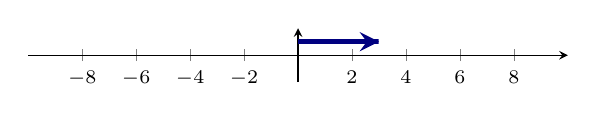
\begin{tikzpicture}
    \begin{axis}[
            xmin=-10,xmax=10,ymin=-1,ymax=1,
            %width=3in,
            clip=false,
            axis lines=center,
            %ticks=none,
            unit vector ratio*=1 1 1,
            ymajorticks=false,
            xtick={-8,-6,-4,-2,2,4,6,8},
            %xlabel=$x$, ylabel=$y$,
            ticklabel style={font=\scriptsize},
            %every axis y label/.style={at=(current axis.above origin),anchor=south},
            every axis x label/.style={at=(current axis.right of origin),anchor=west},
          ]     


            \addplot [line width=2, penColor, smooth,samples=200,domain=(0:3),->] ({x},{0.5});

        \end{axis}
  \end{tikzpicture}
  \end{image}











  \begin{image}
  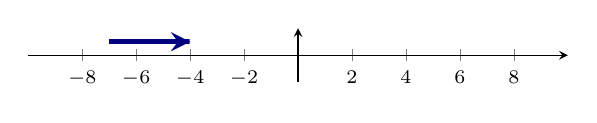
\begin{tikzpicture}
    \begin{axis}[
            xmin=-10,xmax=10,ymin=-1,ymax=1,
            %width=3in,
            clip=false,
            axis lines=center,
            %ticks=none,
            unit vector ratio*=1 1 1,
            ymajorticks=false,
            xtick={-8,-6,-4,-2,2,4,6,8},
            %xlabel=$x$, ylabel=$y$,
            ticklabel style={font=\scriptsize},
            %every axis y label/.style={at=(current axis.above origin),anchor=south},
            every axis x label/.style={at=(current axis.right of origin),anchor=west},
          ]     


            \addplot [line width=2, penColor, smooth,samples=200,domain=(-7:-4),->] ({x},{0.5});

        \end{axis}
  \end{tikzpicture}
  \end{image}






  \begin{image}
  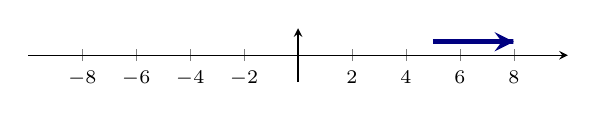
\begin{tikzpicture}
    \begin{axis}[
            xmin=-10,xmax=10,ymin=-1,ymax=1,
            %width=3in,
            clip=false,
            axis lines=center,
            %ticks=none,
            unit vector ratio*=1 1 1,
            ymajorticks=false,
            xtick={-8,-6,-4,-2,2,4,6,8},
            %xlabel=$x$, ylabel=$y$,
            ticklabel style={font=\scriptsize},
            %every axis y label/.style={at=(current axis.above origin),anchor=south},
            every axis x label/.style={at=(current axis.right of origin),anchor=west},
          ]     


            \addplot [line width=2, penColor, smooth,samples=200,domain=(5:8),->] ({x},{0.5});

        \end{axis}
  \end{tikzpicture}
  \end{image}







A negative number is represented by an arrow facing to the left.

These arrows all represent $-3$.








  \begin{image}
  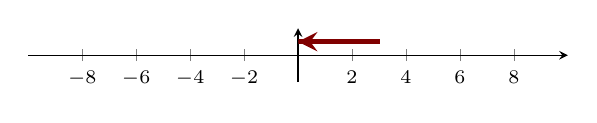
\begin{tikzpicture}
    \begin{axis}[
            xmin=-10,xmax=10,ymin=-1,ymax=1,
            %width=3in,
            clip=false,
            axis lines=center,
            %ticks=none,
            unit vector ratio*=1 1 1,
            ymajorticks=false,
            xtick={-8,-6,-4,-2,2,4,6,8},
            %xlabel=$x$, ylabel=$y$,
            ticklabel style={font=\scriptsize},
            %every axis y label/.style={at=(current axis.above origin),anchor=south},
            every axis x label/.style={at=(current axis.right of origin),anchor=west},
          ]     


            \addplot [line width=2, penColor2, smooth,samples=200,domain=(0:3),<-] ({x},{0.5});

        \end{axis}
  \end{tikzpicture}
  \end{image}











  \begin{image}
  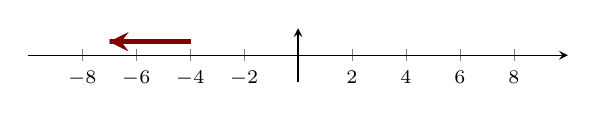
\begin{tikzpicture}
    \begin{axis}[
            xmin=-10,xmax=10,ymin=-1,ymax=1,
            %width=3in,
            clip=false,
            axis lines=center,
            %ticks=none,
            unit vector ratio*=1 1 1,
            ymajorticks=false,
            xtick={-8,-6,-4,-2,2,4,6,8},
            %xlabel=$x$, ylabel=$y$,
            ticklabel style={font=\scriptsize},
            %every axis y label/.style={at=(current axis.above origin),anchor=south},
            every axis x label/.style={at=(current axis.right of origin),anchor=west},
          ]     


            \addplot [line width=2, penColor2, smooth,samples=200,domain=(-7:-4),<-] ({x},{0.5});

        \end{axis}
  \end{tikzpicture}
  \end{image}






  \begin{image}
  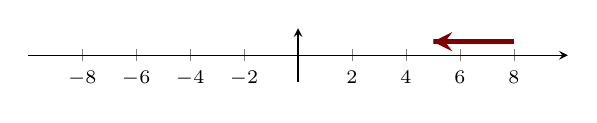
\begin{tikzpicture}
    \begin{axis}[
            xmin=-10,xmax=10,ymin=-1,ymax=1,
            %width=3in,
            clip=false,
            axis lines=center,
            %ticks=none,
            unit vector ratio*=1 1 1,
            ymajorticks=false,
            xtick={-8,-6,-4,-2,2,4,6,8},
            %xlabel=$x$, ylabel=$y$,
            ticklabel style={font=\scriptsize},
            %every axis y label/.style={at=(current axis.above origin),anchor=south},
            every axis x label/.style={at=(current axis.right of origin),anchor=west},
          ]     


            \addplot [line width=2, penColor2, smooth,samples=200,domain=(5:8),<-] ({x},{0.5});

        \end{axis}
  \end{tikzpicture}
  \end{image}







The arrow end of an arrow is called the \textbf{head} and the other end is called the \textbf{tail}.  We envision the arrow encoding the direction going from tail to head.  The direction of the arrow indicates the number's sign.



\subsection*{Operations} 


Arrows help us tell the story of addition and subtraction.



$\blacktriangleright$ \textbf{Addition}


The story of $2+3=5$ as told through arrows is a picture story.  First, an arrow representing $2$ is placed with its tail at $0$.  Secondly, an arrow representing $3$ is placed.  Addition is illustrated by a head-to-tail placement.  Finally, the result is represented by a arrow running from the tail of the first arrow to the head of the second arrow. This arrow is pointing to the right and has a length of $5$.  The result is $5$.




  \begin{image}
  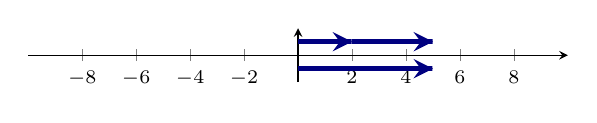
\begin{tikzpicture}
    \begin{axis}[
            xmin=-10,xmax=10,ymin=-1,ymax=1,
            %width=3in,
            clip=false,
            axis lines=center,
            %ticks=none,
            unit vector ratio*=1 1 1,
            ymajorticks=false,
            xtick={-8,-6,-4,-2,2,4,6,8},
            %xlabel=$x$, ylabel=$y$,
            ticklabel style={font=\scriptsize},
            %every axis y label/.style={at=(current axis.above origin),anchor=south},
            every axis x label/.style={at=(current axis.right of origin),anchor=west},
          ]     


            \addplot [line width=2, penColor, smooth,samples=200,domain=(0:2),->] ({x},{0.5});
            \addplot [line width=2, penColor, smooth,samples=200,domain=(2:5),->] ({x},{0.5});

            \addplot [line width=2, penColor, smooth,samples=200,domain=(0:5),->] ({x},{-0.5});

        \end{axis}
  \end{tikzpicture}
  \end{image}





The official mathematical name for an arrow is a \textbf{\textcolor{purple!85!blue}{vector}}.









The story of $2+(-5)=-3$ as told through vectors is a picture story.  First, a vector representing $2$ is placed with its tail at $0$.  Secondly, a vector representing $-5$ is placed.  Addition is illustrated by a head-to-tail placement.  Finally, the result is represented by a vector running from the tail of the first vector to the head of the second vector. This vector is pointing to the left and has a length of $3$.  This vector represents $-3$. The result is $-3$.




  \begin{image}
  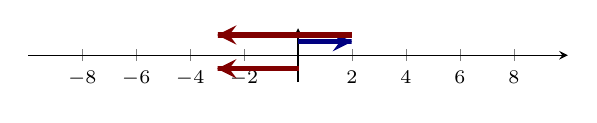
\begin{tikzpicture}
    \begin{axis}[
            xmin=-10,xmax=10,ymin=-1,ymax=1,
            %width=3in,
            clip=false,
            axis lines=center,
            %ticks=none,
            unit vector ratio*=1 1 1,
            ymajorticks=false,
            xtick={-8,-6,-4,-2,2,4,6,8},
            %xlabel=$x$, ylabel=$y$,
            ticklabel style={font=\scriptsize},
            %every axis y label/.style={at=(current axis.above origin),anchor=south},
            every axis x label/.style={at=(current axis.right of origin),anchor=west},
          ]     


            \addplot [line width=2, penColor, smooth,samples=200,domain=(0:2),->] ({x},{0.5});
            \addplot [line width=2, penColor2, smooth,samples=200,domain=(-3:2),<-] ({x},{0.75});

            \addplot [line width=2, penColor2, smooth,samples=200,domain=(-3:0),<-] ({x},{-0.5});

        \end{axis}
  \end{tikzpicture}
  \end{image}















$\blacktriangleright$ \textbf{Subtraction}





The story of $7 - 4 = 3$ as told through vectors is a picture story.  First, an arrow representing $7$ is placed with its tail at $0$.  Secondly, an arrow representing $4$ is also placed with its tail at $0$.  Subtraction is illustrated by a tail-to-tail placement.  Finally, the result is represented by a arrow running from the head of the second vector to the head of the first vector. This vector is pointing to the right and has a length of $3$.  The result is $3$.




  \begin{image}
  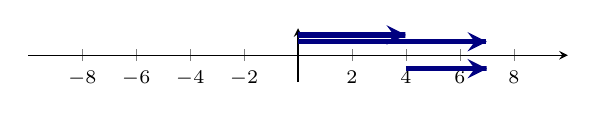
\begin{tikzpicture}
    \begin{axis}[
            xmin=-10,xmax=10,ymin=-1,ymax=1,
            %width=3in,
            clip=false,
            axis lines=center,
            %ticks=none,
            unit vector ratio*=1 1 1,
            ymajorticks=false,
            xtick={-8,-6,-4,-2,2,4,6,8},
            %xlabel=$x$, ylabel=$y$,
            ticklabel style={font=\scriptsize},
            %every axis y label/.style={at=(current axis.above origin),anchor=south},
            every axis x label/.style={at=(current axis.right of origin),anchor=west},
          ]     


            \addplot [line width=2, penColor, smooth,samples=200,domain=(0:7),->] ({x},{0.5});
            \addplot [line width=2, penColor, smooth,samples=200,domain=(0:4),->] ({x},{0.75});

            \addplot [line width=2, penColor, smooth,samples=200,domain=(4:7),->] ({x},{-0.5});

        \end{axis}
  \end{tikzpicture}
  \end{image}







The story of $2-(-3)=5$ as told through vectors is a picture story.  First, an arrow representing $2$ is placed with its tail at $0$.  Secondly, an arrow representing $-3$ is also placed with its tail at $0$.  Subtraction is illustrated by a tail-to-tail placement.  Finally, the result is represented by a arrow running from the head of the second vector to the head of the first vector. This vector is pointing to the right and has a length of $5$.  The result is $5$.




  \begin{image}
  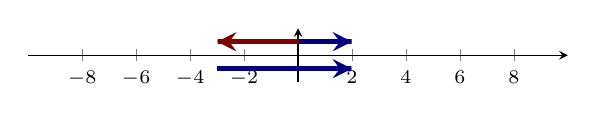
\begin{tikzpicture}
    \begin{axis}[
            xmin=-10,xmax=10,ymin=-1,ymax=1,
            %width=3in,
            clip=false,
            axis lines=center,
            %ticks=none,
            unit vector ratio*=1 1 1,
            ymajorticks=false,
            xtick={-8,-6,-4,-2,2,4,6,8},
            %xlabel=$x$, ylabel=$y$,
            ticklabel style={font=\scriptsize},
            %every axis y label/.style={at=(current axis.above origin),anchor=south},
            every axis x label/.style={at=(current axis.right of origin),anchor=west},
          ]     


            \addplot [line width=2, penColor, smooth,samples=200,domain=(0:2),->] ({x},{0.5});
            \addplot [line width=2, penColor2, smooth,samples=200,domain=(-3:0),<-] ({x},{0.5});

            \addplot [line width=2, penColor, smooth,samples=200,domain=(-3:2),->] ({x},{-0.5});

        \end{axis}
  \end{tikzpicture}
  \end{image}













The story of $-2-(-5)=3$ as told through vectors is a picture story.  First, an arrow representing $-2$ is placed with its tail at $0$.  Secondly, an arrow representing $-5$ is also placed with its tail at $0$.  Subtraction is illustrated by a tail-to-tail placement.  Finally, the result is represented by a arrow running from the head of the second vector to the head of the first vector. This vector is pointing to the right and has a length of $3$.  The result is $3$.




  \begin{image}
  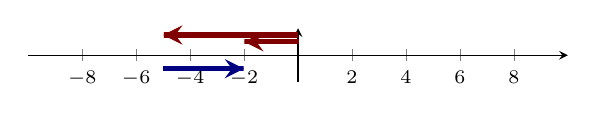
\begin{tikzpicture}
    \begin{axis}[
            xmin=-10,xmax=10,ymin=-1,ymax=1,
            %width=3in,
            clip=false,
            axis lines=center,
            %ticks=none,
            unit vector ratio*=1 1 1,
            ymajorticks=false,
            xtick={-8,-6,-4,-2,2,4,6,8},
            %xlabel=$x$, ylabel=$y$,
            ticklabel style={font=\scriptsize},
            %every axis y label/.style={at=(current axis.above origin),anchor=south},
            every axis x label/.style={at=(current axis.right of origin),anchor=west},
          ]     


            \addplot [line width=2, penColor2, smooth,samples=200,domain=(-2:0),<-] ({x},{0.5});
            \addplot [line width=2, penColor2, smooth,samples=200,domain=(-5:0),<-] ({x},{0.75});

            \addplot [line width=2, penColor, smooth,samples=200,domain=(-5:-2),->] ({x},{-0.5});

        \end{axis}
  \end{tikzpicture}
  \end{image}




From these diagrams we can see that 

\begin{itemize}
\item Addition is commutative.  The head-to-head alignment results in the same arrow regardless of which arrow comes first.
\item Subtraction is not commutative. The tail-to-tail alignment will reverse the resulting arrow if the order is reversed.
\end{itemize}






We want to carry this arrow or vector idea for operations over from 1-dimensional numbers to 2-dimensional numbers.





































\section*{The Plane:  $\mathbb{R}^2 = \mathbb{R} \times \mathbb{R}$}




We would like to extend this picture system from one copy of \textbf{$\mathbb{R}$} to two copies of \textbf{$\mathbb{R}$}. \\

\textbf{$\mathbb{R} \times \mathbb{R}$} is shorthand notation for two copies of the real line forming the Cartesian plane.  \textbf{$\mathbb{R}^2$} is even shorter shorthand notation.

$\mathbb{R}^2$ is just the collection of ordered pairs of real numbers.

\[  \mathbb{R}^2 = \{  (r_1, r_2)    \, | \,  r_1, r_2 \in \mathbb{R}  \}      \]


The Cartesian plane is our geometric, visual representation of these ordered pairs. We can plot points or dots to represent a 2-dimensional number.



Plotting dots for the numbers $(-4,7)$, $(3,5)$, $(5,-6)$, and $(-7,-3)$.

\begin{image}
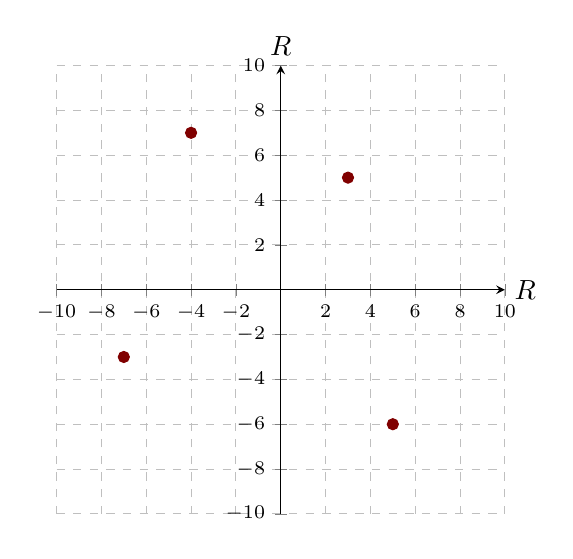
\begin{tikzpicture}
  \begin{axis}[
            domain=-10:10, ymax=10, xmax=10, ymin=-10, xmin=-10,
            axis lines =center, xlabel=$\mathbb{R}$, ylabel=$\mathbb{R}$, grid = major, grid style={dashed},
            unit vector ratio*=1 1 1,
            ytick={-10,-8,-6,-4,-2,2,4,6,8,10},
            xtick={-10,-8,-6,-4,-2,2,4,6,8,10},
            yticklabels={$-10$,$-8$,$-6$,$-4$,$-2$,$2$,$4$,$6$,$8$,$10$}, 
            xticklabels={$-10$,$-8$,$-6$,$-4$,$-2$,$2$,$4$,$6$,$8$,$10$},
            ticklabel style={font=\scriptsize},
            every axis y label/.style={at=(current axis.above origin),anchor=south},
            every axis x label/.style={at=(current axis.right of origin),anchor=west},
            axis on top
          ]
          
            \addplot [color=penColor2,only marks,mark=*] coordinates{(-4,7)};
            \addplot [color=penColor2,only marks,mark=*] coordinates{(3,5)};
            \addplot [color=penColor2,only marks,mark=*] coordinates{(5,-6)};
            \addplot [color=penColor2,only marks,mark=*] coordinates{(-7,-3)};

  \end{axis}
\end{tikzpicture}
\end{image}




We now have a 2-dimensional number line.








\textbf{\textcolor{red!25!blue!75!}{2D Operations}} \\



We now enhance the plane with an arithmetic.  We are just going to adopt the arrow rules.  

\textbf{Step 1)} Convert each dot to an arrow.


$\blacktriangleright$ \textbf{Addition:}  Draw the first arrow with its tail at the origin.  Draw the second arrow head-to-tail. The  resulting arrow is drawn from the tail of the first arrow to the head of the second arrow.  This resulting arrow represents the sum of the two 2D-numbers.




\begin{example}


$(4,6) + (2, -10)$


\begin{image}
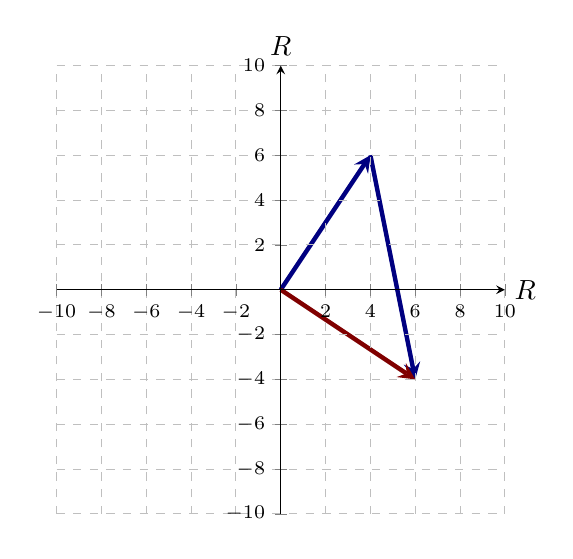
\begin{tikzpicture}
  \begin{axis}[
            domain=-10:10, ymax=10, xmax=10, ymin=-10, xmin=-10,
            axis lines =center, xlabel=$\mathbb{R}$, ylabel=$\mathbb{R}$, grid = major, grid style={dashed},
            unit vector ratio*=1 1 1,
            ytick={-10,-8,-6,-4,-2,2,4,6,8,10},
            xtick={-10,-8,-6,-4,-2,2,4,6,8,10},
            yticklabels={$-10$,$-8$,$-6$,$-4$,$-2$,$2$,$4$,$6$,$8$,$10$}, 
            xticklabels={$-10$,$-8$,$-6$,$-4$,$-2$,$2$,$4$,$6$,$8$,$10$},
            ticklabel style={font=\scriptsize},
            every axis y label/.style={at=(current axis.above origin),anchor=south},
            every axis x label/.style={at=(current axis.right of origin),anchor=west},
            axis on top
          ]


            \draw[penColor,ultra thick,->] (axis cs:0,0) -- (axis cs:4,6);
            \draw[penColor,ultra thick,->] (axis cs:4,6) -- (axis cs:6,-4);
            \draw[penColor2,ultra thick,->] (axis cs:0,0) -- (axis cs:6,-4);



  \end{axis}
\end{tikzpicture}
\end{image}


$(4,6) + (2, -10) = (6, -4)$


\end{example}







$\blacktriangleright$ \textbf{Subtraction:}  Draw the first arrow with its tail at the origin.  Draw the second arrow with its tail at the origin. The resulting arrow is drawn from the head of the second arrow to the head of the first arrow.  This resulting arrow represents the difference of the two 2D-numbers.






\begin{example}


$(4,6) - (2, -10)$


\begin{image}
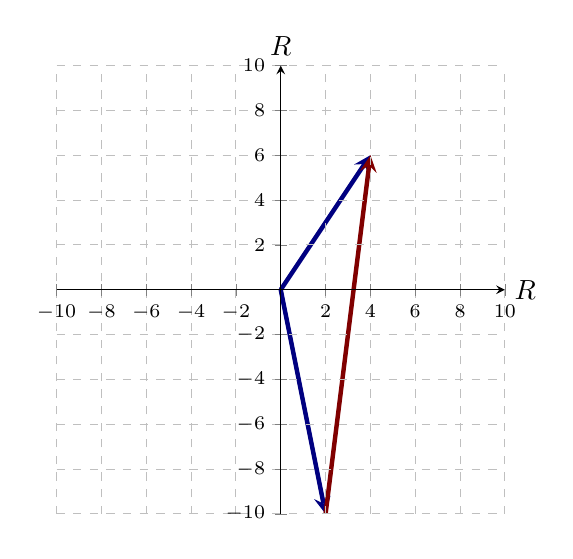
\begin{tikzpicture}
  \begin{axis}[
            domain=-10:10, ymax=10, xmax=10, ymin=-10, xmin=-10,
            axis lines =center, xlabel=$\mathbb{R}$, ylabel=$\mathbb{R}$, grid = major, grid style={dashed},
            unit vector ratio*=1 1 1,
            ytick={-10,-8,-6,-4,-2,2,4,6,8,10},
            xtick={-10,-8,-6,-4,-2,2,4,6,8,10},
            yticklabels={$-10$,$-8$,$-6$,$-4$,$-2$,$2$,$4$,$6$,$8$,$10$}, 
            xticklabels={$-10$,$-8$,$-6$,$-4$,$-2$,$2$,$4$,$6$,$8$,$10$},
            ticklabel style={font=\scriptsize},
            every axis y label/.style={at=(current axis.above origin),anchor=south},
            every axis x label/.style={at=(current axis.right of origin),anchor=west},
            axis on top
          ]


            \draw[penColor,ultra thick,->] (axis cs:0,0) -- (axis cs:4,6);
            \draw[penColor,ultra thick,->] (axis cs:0,0) -- (axis cs:2,-10);
            \draw[penColor2,ultra thick,->] (axis cs:2,-10) -- (axis cs:4,6);



  \end{axis}
\end{tikzpicture}
\end{image}


$(4,6) - (2, -10) = (2, 16)$


\end{example}














This discussion is very suggestive of a symbolic version of 2-dimensional addition and subtraction.







\section*{Vectors}


The arrow combination suggest an algebraic description.

$(4,6) + (2, -10) = (4+2, 6+(-10))  = (6, -4)$



Except, we are already using the parentheses to represent points or dots.




\begin{image}
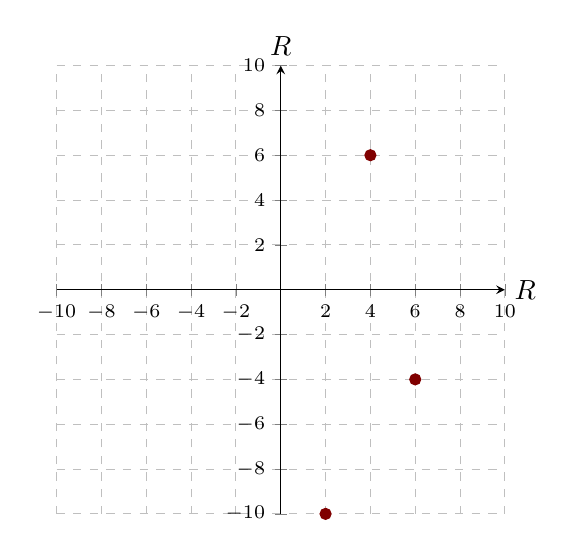
\begin{tikzpicture}
  \begin{axis}[
            domain=-10:10, ymax=10, xmax=10, ymin=-10, xmin=-10,
            axis lines =center, xlabel=$\mathbb{R}$, ylabel=$\mathbb{R}$, grid = major, grid style={dashed},
            unit vector ratio*=1 1 1,
            ytick={-10,-8,-6,-4,-2,2,4,6,8,10},
            xtick={-10,-8,-6,-4,-2,2,4,6,8,10},
            yticklabels={$-10$,$-8$,$-6$,$-4$,$-2$,$2$,$4$,$6$,$8$,$10$}, 
            xticklabels={$-10$,$-8$,$-6$,$-4$,$-2$,$2$,$4$,$6$,$8$,$10$},
            ticklabel style={font=\scriptsize},
            every axis y label/.style={at=(current axis.above origin),anchor=south},
            every axis x label/.style={at=(current axis.right of origin),anchor=west},
            axis on top
          ]

            \addplot [color=penColor2,only marks,mark=*] coordinates{(4,6)};
            \addplot [color=penColor2,only marks,mark=*] coordinates{(2,-10)};
            \addplot [color=penColor2,only marks,mark=*] coordinates{(6,-4)};



  \end{axis}
\end{tikzpicture}
\end{image}




We need new words and symbols.




A \textbf{vector} is going to play the part of a number.  We'll represent vectors with arrows. Just like on the 1-dimensional number line, vectors don't have a position.  They have a length and a direction.  Many arrows drawn at different positions on the plane could represent the same vector.

We'll use \textbf{triangular brackets} as algebraic notation for vectors. 

Example:  $\langle 4, 5 \rangle$












\begin{center}
\textbf{\textcolor{green!50!black}{ooooo-=-=-=-ooOoo-=-=-=-ooooo}} \\

more examples can be found by following this link\\ \link[More Examples of Representing Numbers]{https://ximera.osu.edu/csccmathematics/precalculus2/precalculus2/representingNumbers/examples/exampleList}

\end{center}








\end{document}
